\documentclass[a4paper,11pt]{article}

\input ../include/preamble.tex

\usepackage{tikz}
\usetikzlibrary{automata,arrows,topaths,calc,positioning}

\usepackage{subcaption}

\usepackage{changepage}

\usepackage{listings}

\lstdefinelanguage{elixir}{
	morekeywords={case,catch,def,do,else,false,%
		use,alias,receive,timeout,defmacro,defp,%
		for,if,import,defmodule,defprotocol,%
		nil,defmacrop,defoverridable,defimpl,%
		super,fn,raise,true,try,end,with,%
		unless},
	otherkeywords={<-,->},
	sensitive=true,
	morecomment=[l]{\#},
	morecomment=[n]{/*}{*/},
	morestring=[b]",
	morestring=[b]',
	morestring=[b]"""
}

\lstset{language=elixir}

\begin{document}

\title{
    \textbf{An exercise in communication}\\
    \large{Programming II - Elixir Version}
}
\author{Johan Montelius}
\date{Spring Term 2018}
\maketitle
\defaultpagestyle

\section*{Introduction}

This exercise is partly about breaking up a problem in layers of
abstractions and implement each layer as a process or a set of
processes. We will model our solution as communicating finite state
machines and each machine is of course implemented as an Elixir
process.

The problem that we will look at is how to create a communication
abstraction that provides addressing and FIFO delivery over a lossy
channel. The situation will look similar to that of TCP/IP but our
problem statement and solution will be much simpler.

\section{A transport abstraction}

Assume that we want to create a {\em transport service}. The service
should provide the following functionality:

\begin{itemize}

\item identity: The service should provide addresses, we should
  be able to send and receive messages to other processes given an
  address.

\item flow control: The service should take care of flow control so
  we should not be able to send more messages than the receiver can
  consume.

\item ordered delivery: Packets should be delivered in order.

\item reliable delivery: Packets should be delivered even if the
  underlying communication channel is lossy.

\end{itemize}

This is not that hard to achieve and the solution could easily be be
described in a state diagram with 15 states and 123
transitions..... The problem we would have is that, if we want to solve
all these properties in one go, we would have so many things to keep
track of that the solution would look like a bowl of spaghetti.

Instead of solving all problems at once we divide the solution into
layers, each layer providing a service that brings us closer to the
final solution. The layers that we will implement have similarities
with the ISO communication layers or the layers in the IP stack. The
layers that we will work with are:

\begin{itemize}

\item link: This layer is given, it will send a {\em frame} on a
  wire but does not know very much more. There are no guarantees that the
  frame will arrive nor that frames will arrive in order.

\item network: This layer will introduce {\em network addresses} so we
  can have several nodes connected together. It uses the link layer
  straight off so we do not add ordered delivery nor guarantees of
  message delivery.

\item order: This layer will add re-transmissions of
  missing messages and keep track of ordering of messages. 
  
\item flow: This layer will solve the flow-control problem.

\end{itemize}

The TCP protocol is similar to our order and flow layers but also
implements congestion avoidance, process addressing, stream to datagram
segmentation etc. In this implementation we only provide reliability
and flow control to make things a bit easier. We will also implement
them as separate layers to show how simple each layer can be
implemented.

If we draw a diagram over the complete system it will look like
Fig.\ref{fig:arch}. Each layer will have one or more processes that
implements the right abstractions. In its first incarnation each layer
will be handled by a single process but when we extend the system we
might want to have separate processes for different directions.

\begin{figure}
  \centering
  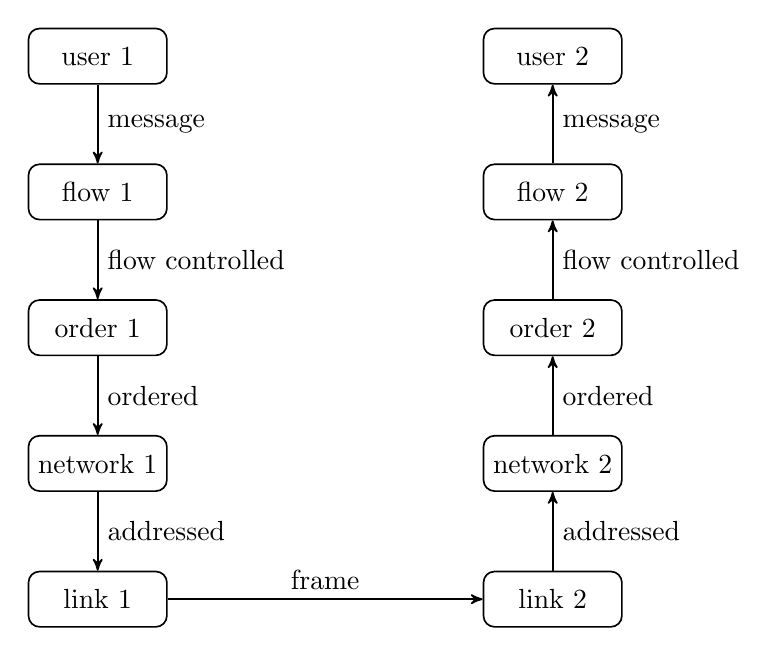
\begin{tikzpicture}[>=stealth', semithick, auto]

    \tikzstyle{fbp} = [rectangle, rounded corners, minimum width=50pt, minimum height=20pt, text centered, draw=black]        


    \node (user1)  [fbp]                                 {user 1};
    \node (user2)  [fbp, right=4cm of user1]             {user 2};            
    
    \node (flow1)  [fbp, below=1cm of user1]             {flow 1};
    \node (flow2)  [fbp, below=1cm of user2]             {flow 2};        

    \node (order1) [fbp, below=1cm of flow1]             {order 1};
    \node (order2) [fbp, below=1cm of flow2]             {order 2};        

    \node (netw1)  [fbp, below=1cm of order1]            {network 1};
    \node (netw2)  [fbp, below=1cm of order2]            {network 2};

    \node (link1)  [fbp, below=1cm of netw1]             {link 1};
    \node (link2)  [fbp, below=1cm of netw2]             {link 2};    

    \path[->]  (user1)    edge        node         {message}       (flow1);
    \path[<-]  (user2)    edge        node         {message}       (flow2);
    
    \path[->]  (flow1)    edge        node         {flow controlled}       (order1);
    \path[<-]  (flow2)    edge        node         {flow controlled}       (order2);
    
    \path[->]  (order1)   edge        node         {ordered}       (netw1);
    \path[<-]  (order2)   edge        node         {ordered}       (netw2);

    \path[->]  (netw1)   edge        node          {addressed}       (link1);
    \path[<-]  (netw2)   edge        node          {addressed}       (link2);

    \path[->]  (link1)   edge        node          {frame}       (link2);
  \end{tikzpicture}

  \caption{The architecture.}
  \label{fig:arch}
      
\end{figure}

We now start form the ground up and implement layer by layer. We
should be able to test that a layer works before implementing the next
layer.

\section{link layer}

The link layer process is, as shown in Fig.\ref{fig:link} quite
simple. We will first start the process and give it the process
identifier of the master process. We will then send it a message that
connect the process with a destination link layer process. 

\begin{figure}
\centering  
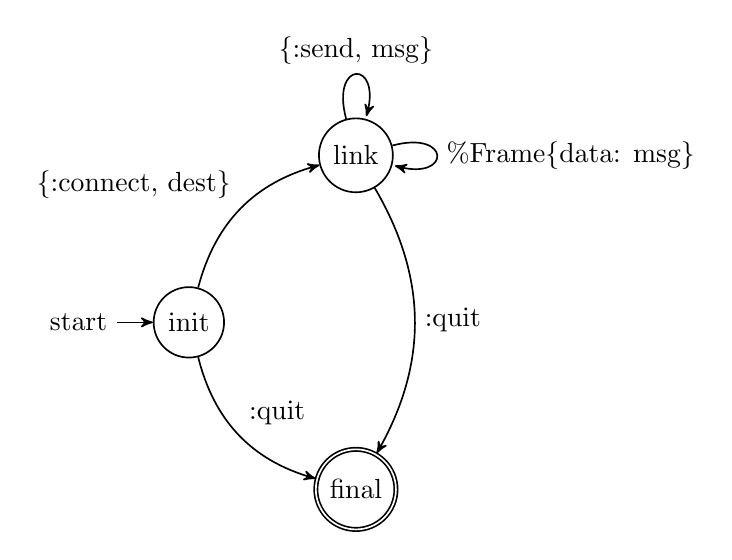
\begin{tikzpicture}[>=stealth', node distance=3cm, semithick, auto]

    \node[initial, state]            (init)                              {init};
    \node[state]                     (link)    [above right of=init]     {link};
    \node[accepting, state]          (final)   [below right of=init]     {final};


    \path[->]   (init)   edge       [bend left]     node      {\{:connect, dest\}}       (link)
                         edge       [bend right]    node      {:quit}          (final) 
                (link)   edge       [loop above]    node      {\{:send, msg\}}          (link)
                         edge       [loop right]    node      {\%Frame\{data: msg\}}           (link)
                         edge       [bend left]     node      {:quit}          (final);
\end{tikzpicture}

\caption{The link layer.}
\label{fig:link}

\end{figure}

Note the order here; we can not provide the link layer process with
its connection point when we create the process. If we tried we would
end up in a chicken or the egg question. We solve this by first
creating both link processes and the send them a message with the process
identifier of their peer.

The link layer should be able to handle the following messages:

\begin{itemize}

\item {\tt \{:send, msg\} }: A message from the master (the network
  layer process), telling the link process to send the message, {\tt
    msg}, to the destination process. The message is wrapped in a {\em
    Frame} and sent using the regular Elixir send primitive.

  \item {\tt \%Frame\{data: msg\}}: A frame from the peer  link
    process. This message should be forwarded to the master process
    using the regular Elixir send primitive. The message is sent as
    is, {\tt msg}, without being wrapped in any special data structure.
\end{itemize}

The Elixir implementation is given in Appendix \ref{app:link}. Before
we continue we write a small test program and connect two nodes
together.

\begin{minted}{elixir}
  def test_link() do
    sender = spawn(fn() -> sender() end)
    receiver = spawn(fn() -> receiver() end)
    {:ok, ls} = Link.start(sender)
    {:ok, lr} = Link.start(receiver)
    send(ls,{:connect, lr})
    send(lr, {:connect, ls})
    send(sender, {:connect, ls})
    send(receiver, {:connect, lr})
    :ok
  end
\end{minted}

This program will start two processes, the {\tt sender} and the {\tt
  receiver};  note the order in which we have to start the
processes. The two master processes are started first in order to
provide the link processes with their respective master. Once the link
processes are created we can connect them together and then connect
the master processes to the link processes.

The {\tt link\_sender} process could look like follows. Implement the
corresponding receive process and see if your systems runs.

\begin{minted}{elixir}
def sender() do
  receive do
    {:connect, lnk} ->
      :io.format("sender connected to link ~w ~n", [lnk]),
      :io.format("sending hello~n", [])
      send(lnk, {:send, :hello})
  end
end            
\end{minted}

\section{a hub}

If we only have two nodes in our network it is rather pointless, so we
will implement a ``hub'' to which we can connect several nodes. The
hub will accept new connection and forward incoming frames to all
connected nodes. The state machine is shown in Fig.~\ref{fig:hub}. In
the implementation we only need to solve how connections should be
stored and how to implement broadcasting of messages.

As an extra precaution we add monitoring of connected link layer processes. If a
process dies we remove it from the set of connected
processes. This will save the state of the hub from growing in an
environment where nodes fail before having been disconnected.

An implementation can be found in Appendix \ref{app:link}. Write a
small test program, similar to the previous one, where two link layer
processes are connected using a hub.

\begin{figure}
\centering  
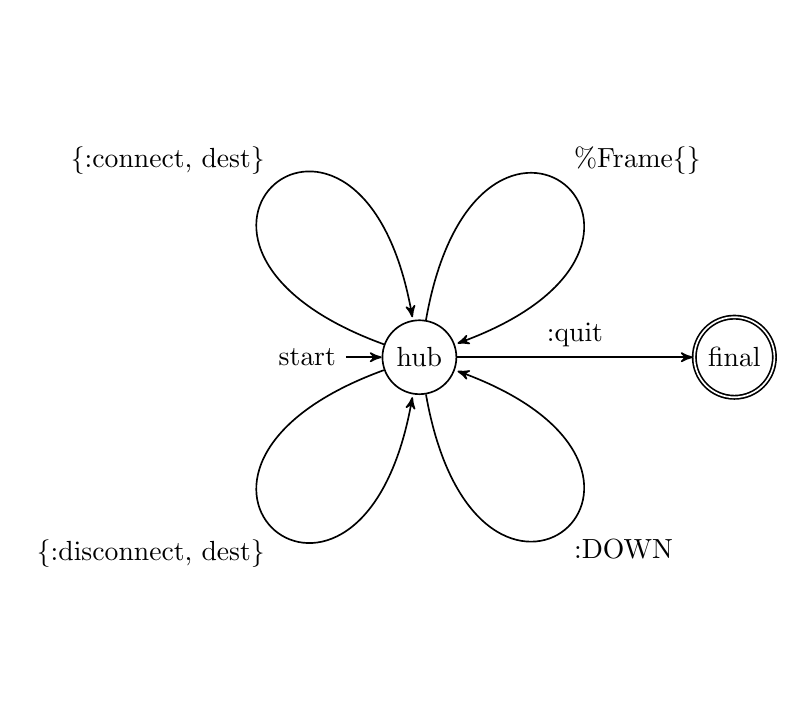
\begin{tikzpicture}[>=stealth', node distance=4cm, semithick, auto]

    \node[initial, state]            (hub)                        {hub};
    \node[accepting, state]          (final)   [right of=hub]     {final};


    
    \path[->]   (hub)   edge       [loop above, every loop/.append style={looseness=20,in=100, out=160 }]    node[anchor=south east]      {\{:connect, dest\}}       (hub)
                        edge       [loop below, every loop/.append style={looseness=20,in=260, out=200 }]    node[anchor=north east]      {\{:disconnect, dest\}}    (hub)
                        edge       [loop above, every loop/.append style={looseness=20,in=20,  out=80 }]     node[anchor=south west]      {\%Frame\{\}}              (hub)
                        edge       [loop below, every loop/.append style={looseness=20,in=340, out=280 }]    node[anchor=north west]      {:DOWN}                    (hub)
                        edge       []                                                                        node      {:quit}                    (final);
    

\end{tikzpicture}
\caption{The hub.}
\label{fig:hub}
\end{figure}


\section{network layer}

So we now have a link layer that works but the thing is that the hub
will happily broadcast any message to all connected nodes. If we
connect three nodes to the hub all three nodes will receive all
messages. We need a network layer that introduces an addressing scheme
so we can send a message to a particular node in the network.

In Fig.\ref{fig:net} we have the state diagram of the network layer
and as you see it is not much more complicated than then link
layer. You might wonder why we did not implement the network layer
directly since the link layer does not give us any thing besides
message delivery but we might want to add more features, such as error
detection, in the link layer and want to be able to do this without
modifying the network layer.

\begin{figure}
\centering  
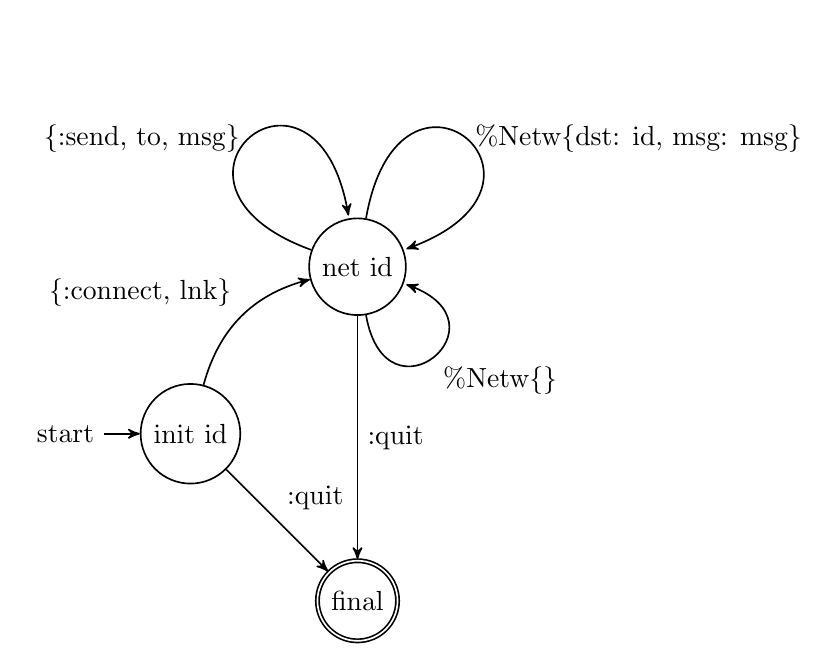
\begin{tikzpicture}[>=stealth', node distance=3cm, semithick, auto]

    \node[initial, state]   (init)                             {init id};
    \node[state]            (net)    [above right of=init]     {net id};
    \node[accepting, state] (final)  [below right of=init]     {final};

    
    \path[->]   (init)   edge       [bend left]     node      {\{:connect, lnk\}}       (net)
                         edge       []             node       {:quit}                   (final)
                (net)    edge       [loop above, every loop/.append style={looseness=10,in=20, out=80 }]   node[anchor=west] {\%Netw\{dst: id, msg: msg\}}(net)
                         edge       [loop above, every loop/.append style={looseness=10,in=100, out=160 }] node[anchor=east] {\{:send, to, msg\}}    (net)
                         edge       [loop below, every loop/.append style={looseness=6,in=340, out=280 }]  node[anchor=north west] {\%Netw\{\}}             (net)
                         edge       []                                                                     node              {:quit}                 (final);
    
\end{tikzpicture}
\caption{The network layer.}
\label{fig:net}
\end{figure}

The network layer is given a unique identifier when it is started and
it will use this address to filter incoming messages. When we start
the process we also provide its master process so that it knows to whom
it should redirect incoming messages. Before we start sending messages
we connect the processes to a link layer process; following the
same pattern as for the test procedures for the link layer.


In Appendix \ref{app:netw} you will find an implementation of a
network layer process. Implement a simple test function that as before
creates a sender and receiver process that are connected using two
network layer processes. The tricky part is how to start the processes
in the right order: application layer, network layer, link layer,
connect link layers, connect network layer to link layer, connect
application layer to network layer.


\section{order and reliability}

In the next layer we will create a process for one particular flow of
messages. We will then make sure that these messages are delivered
properly by adding a sequence number to the messages and re-transmit
messages that could be lost.

If messages can come out of order we need a way to
impose some order. The ordering is solved if the sending process
numbers the messages as they are sent and the receiver will buffer
received messages and deliver them in the right order. 

A problem occurs if a message is lost; if we do not do anything to
solve this the receiver will wait forever for a message that will
never arrive. The solution is of course to let the sender keep a copy
of each message in case it is lost and to let the receiver request a
re-transmission. This can be solved either by explicitly request
transmissions or by acknowledge messages that do arrive correctly, we
will choose the latter alternative.

To understand how the layer works we describe the process of a sender
process and the receiver process as two different state machines. In
the implementation we will however combine these machines into one
Elixir process.

\begin{figure}
\begin{adjustwidth}{-3cm}{-3cm}
\centering
\begin{subfigure}[b]{6cm}
\resizebox{6cm}{!}{
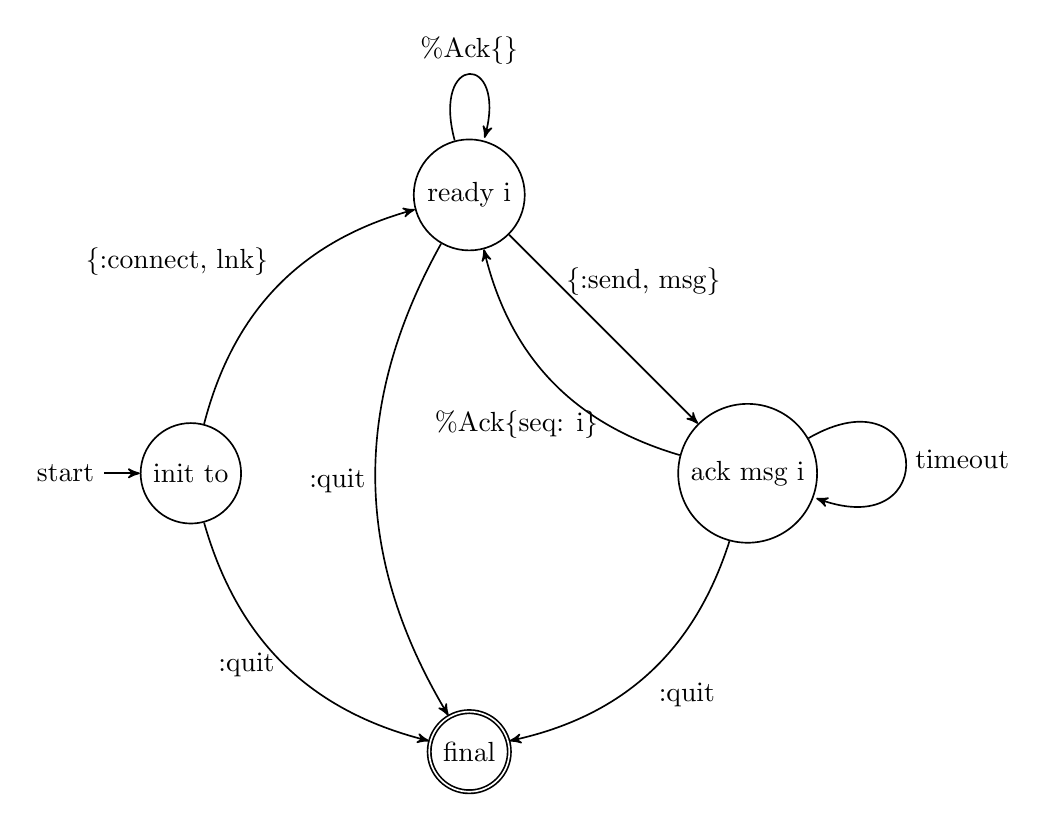
\begin{tikzpicture}[scale=1, >=stealth', node distance=5cm, semithick, auto]
    \node[initial, state]            (init)                              {init to};
    \node[state]                     (ready)   [above right of=init]     {ready i};
    \node[state]                     (send)    [below right of=ready]    {ack msg i};
    \node[accepting, state]          (final)   [below right of=init]     {final};

    
    \path[->]   (init)   edge       [bend left]  node                          {\{:connect, lnk\}}   (ready)
                         edge       [bend right] node[anchor=east]             {:quit}               (final)
                (ready)  edge       []           node[anchor=west, near start] {\{:send, msg\}}      (send)
                         edge       [loop above] node                          {\%Ack\{\}}         (ready)
                         edge       [bend right] node[anchor=east]             {:quit}               (final)                   
                (send)   edge       [loop below, every loop/.append style={looseness=6,in=340, out=30 }] node[anchor=west] {timeout}  (send)   
                         edge       [bend left]  node[near start, anchor=east]              {\%Ack\{seq: i\}}          (ready)
                         edge       [bend left]  node                          {:quit}               (final);
\end{tikzpicture}}
\subcaption{sending process}
\end{subfigure}\qquad%
\begin{subfigure}[b]{6cm}
\resizebox{6cm}{!}{
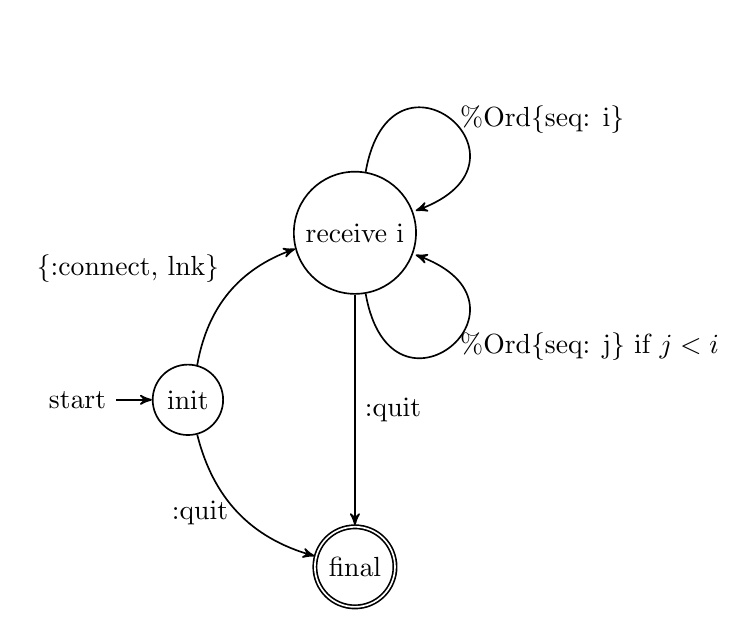
\begin{tikzpicture}[scale=1,>=stealth', node distance=3cm, semithick, auto]
    \node[initial, state]            (init)                              {init};
    \node[state]                     (receive) [above right of=init]     {receive i};
    \node[accepting, state]          (final)   [below right of=init]     {final};

    
    \path[->]   (init)   edge       [bend left]                  node              {\{:connect, lnk\}}   (receive)
                         edge       [below, bend right]          node[anchor=east] {:quit}               (final)
               (receive)   edge     [loop above, every loop/.append style={looseness=6,in=20, out=80}]   node[anchor=west] {\%Ord\{seq: i\}} (receive)
                         edge       [loop below, every loop/.append style={looseness=6,in=340, out=280}] node[anchor=west] {\%Ord\{seq: j\} if $j<i$}  (receive)
                         edge       []                                                                   node              {:quit}                   (final);
\end{tikzpicture}}
\subcaption{receiving process}
\end{subfigure}

\caption{The ordering layer.}
\label{fig:order}
\end{adjustwidth}
\end{figure}

In Fig.\ref{fig:order} we see the state machines of the sender and
receiver processes. This description in simplified in that it will
only allow one outstanding message. The sender will be directed to
send a message to the receiver and will move in to a state where it is
waiting for an {\em acknowledgement} for that particular message {\em
  i}. If everything works it will receive the {\em Ack} message and go
back to the ready state. If no acknowledge message is received it will
receive a timeout and resend the message ({\em msg}).

The receiver knows what sequence number it is waiting. When the
correct message arrives it will send an acknowledge message in return
and forward it to its master. It could be that the sender has already
sent a copy of the message so it must be prepared to discard messages
that it has already seen. The sender must likewise be prepared to
discard {\em Ack} messages that it has seen.

Both processes are started and given a specified network address that
it is communication with. It is then given access to a network process
to use when sending messages. The network processes have addresses and
we here assume that the sender and receiver are the only processes
that are communicating using these addresses. The network processes are
thus dedicated to this communication channel.

In this simple version we only allow one message to be outstanding at
any given time. Only when a message has been acknowledged will we send
the next message. This is of course a severe limitation; our
communication channel will be depending on the round trip thus being
very slow.

To solve this we extend the sender, as shown in
Fig.~\ref{fig:multiple}, to allow several outstanding messages at the
same time. We extend the receive {\em ack} state so that we
can send new messages while we are waiting for an acknowledgment. We
have too keep track of all sent messages and make sure that we resend
the right one so we keep all sent messages, with their corresponding
sequence number, in a buffer (an list of all messages with the last
message sent last).

The sender can now receive the following messages:

\begin{itemize}
\item {\tt \{:send, msg\}}: The process will send the message in a
  numbered datagram to the receiving process. It will store the
  message with its corresponding sequence number as the last element in
  the buffer. The sequence number is then updated.

\item {\tt \%Ack\{seq: a\}}: if $a$
  is equal to the sequence number of the first element in the buffer
  then this element is removed from the buffer.If we receive an
  acknowledgment and remove the last element from the buffer we move
  to the {\em ready} state.

\item {\tt \%Ack\{seq: a\}}: if $a$ is less than the sequence number
  of the first element in the buffer, this is a duplicate
  acknowledgment and can be ignored.

\item {\tt timeout} : the process will resend the first element in the buffer.

\end{itemize}


Note that we have excluded one alternative from the description. A
sending process can send messages $14$, $15$ and $16$,
and then receive an acknowledgment for $15$
- what should we do? We could of course remove the element from the
buffer immediately but in our description we defer the message until
$15$ is the first element in the buffer. Implicit deferral is a technique
that allows us to simplify the description but it also introduce
complications that we will discuss later.


\begin{figure}
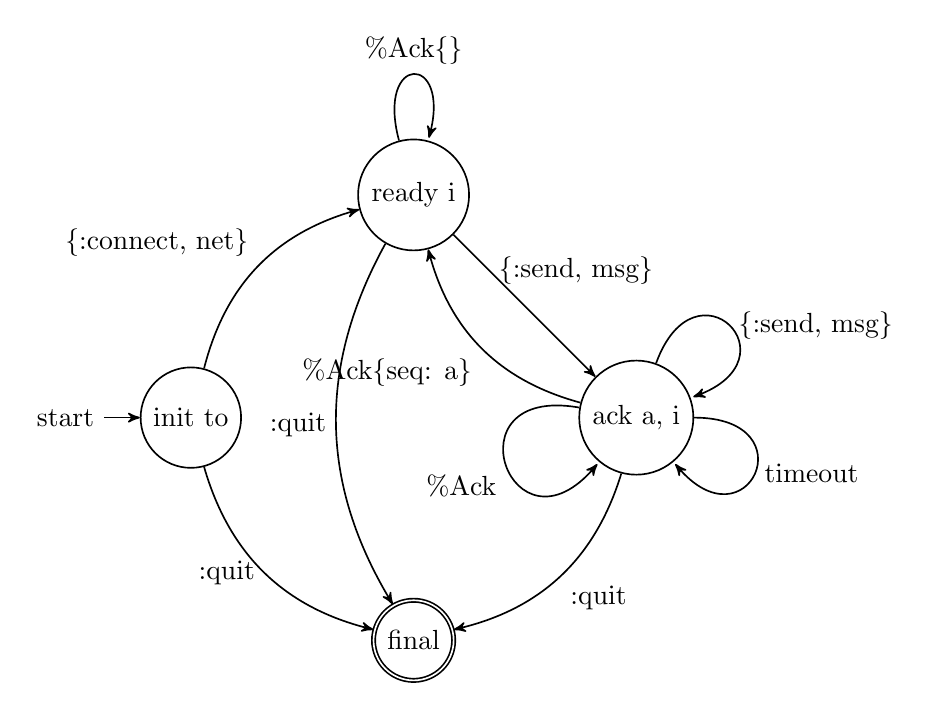
\begin{tikzpicture}[scale=1, >=stealth', node distance=4cm, semithick, auto]
    \node[initial, state]            (init)                              {init to};
    \node[state]                     (ready)   [above right of=init]     {ready i};
    \node[state]                     (send)   [below right of=ready]     {ack a, i};
    \node[accepting, state]          (final)   [below right of=init]     {final};

    
    \path[->]   (init)   edge       [bend left]   node                          {\{:connect, net\}}       (ready)
                         edge       [bend right]  node[anchor=east]             {:quit}                   (final)
                (ready)  edge       []            node[anchor=west, near start] {\{:send, msg\}}          (send)
                         edge       [loop above]  node                          {\%Ack\{\}}               (ready)
                         edge       [bend right]  node[anchor=east]             {:quit}                   (final)                   
                (send)   edge       [loop above, every loop/.append style={looseness=6,in=20, out=70 }]   node[anchor=west]    {\{:send, msg\}} (send)
                         edge       [loop below, every loop/.append style={looseness=6,in=310, out=0 }]   node[anchor=west]    {timeout}        (send)   
                         edge       [loop above, every loop/.append style={looseness=6,in=230, out=170 }] node[anchor=north east]   {\%Ack{}}        (send)
                         edge       [bend left]   node  {\%Ack\{seq: a\}}  (ready)
                         edge       [bend left]   node  {:quit}            (final);
\end{tikzpicture}
\caption{The ordering process: multiple outstanding messages.}
\label{fig:multiple}
\end{figure}

In the description we have chosen to describe the sender and the
receiver as two state machines, which they are. In the implementation
however, we will implement them both as one Elixir process in the same
way as we have implemented the link layer or network layer. We do this
in order to provide a duplex communication channel without having to
create two pairs or processes for each direction. The implementation
becomes trickier since we now have to keep track of both outstanding
buffered messages as well as what messages to receive and acknowledge.


\section{flow control layer}

The next layer will be slightly different since we now will do
synchronous reads of messages. The previous layers have simply passed
an incoming message to the master process but now we require the
master process to actively do a read operations. Similarly the send
operation is acknowledged so the user of the sending process knows
that it is safe to send the next message. The application layer thus
has a message interface that looks like follows:

\begin{itemize}
\item {\tt \{:send, msg, pid\}} : sent to the sending process, a {\tt
    :ok} message is delivered to the process {\tt pid}, when its safe
  to send the next message.

\item {\tt \{:read, n, pid\}} : sent to the reading process, at most
  {\tt n} messages are returned in a message {\tt \{:ok, l, mgs\}}
  where {\tt l} is the number of messages.
\end{itemize}

This layer would be easy to implement if we only allowed one
outstanding message but we would of course like to implement a
buffered system to increase the throughput. The read process thus keeps
a buffer of incoming messages that are waiting to be read. The buffer
does of course have a maximum size and the sender must be careful not
to overflow the reader with messages. Before the sender can start to
send messages it must therefore receive a {\em synchronize} message
that informs the sender of how many more messages it can send. In the
first message the reader informs the sender of the maximum size of the
buffer and it is then the responsibility of the sender to keep track of
how many more messages it can send.


\begin{figure}
\begin{adjustwidth}{-3cm}{-3cm}

\centering
\begin{subfigure}[b]{6cm}
\resizebox{6cm}{!}{
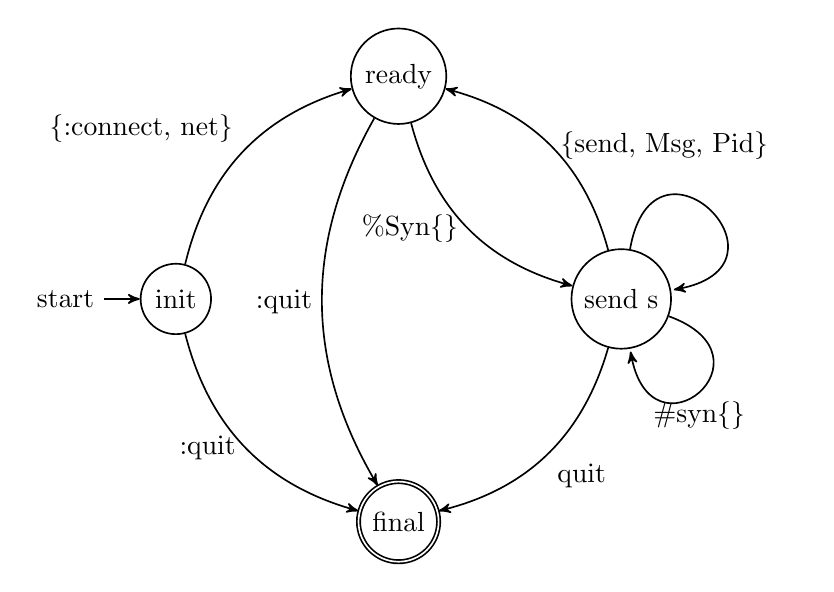
\begin{tikzpicture}[scale=1, >=stealth', node distance=4cm, semithick, auto]
    \node[initial, state]            (init)                              {init};
    \node[state]                     (ready)   [above right of=init]     {ready};
    \node[state]                     (send)   [below right of=ready]     {send s};
    \node[accepting, state]          (final)   [below right of=init]     {final};

    
    \path[->]   (init)   edge       [bend left]  node               {\{:connect, net\}}       (ready)
                         edge       [bend right] node[anchor=east]  {:quit}                   (final)
                (ready)  edge       [bend right] node[anchor=east]  {\%Syn\{\}}               (send)
                         edge       [bend right] node[anchor=east]  {:quit}                   (final)                   
                (send)   edge       [bend right] node[anchor=west]  {\{send, Msg, Pid\}}  (ready)
                         edge       [loop below, every loop/.append style={looseness=6,out=80, in=10 }]   node[anchor=east]  {}              (send)   
                         edge       [loop below, every loop/.append style={looseness=6,out=340, in=280 }] node[anchor=north] {\#syn\{\}}     (send)
                         edge       [bend left]               node       {quit}          (final);
\end{tikzpicture}}
\subcaption{sending process}
\end{subfigure}\qquad%
\begin{subfigure}[b]{6cm}
\resizebox{6cm}{!}{
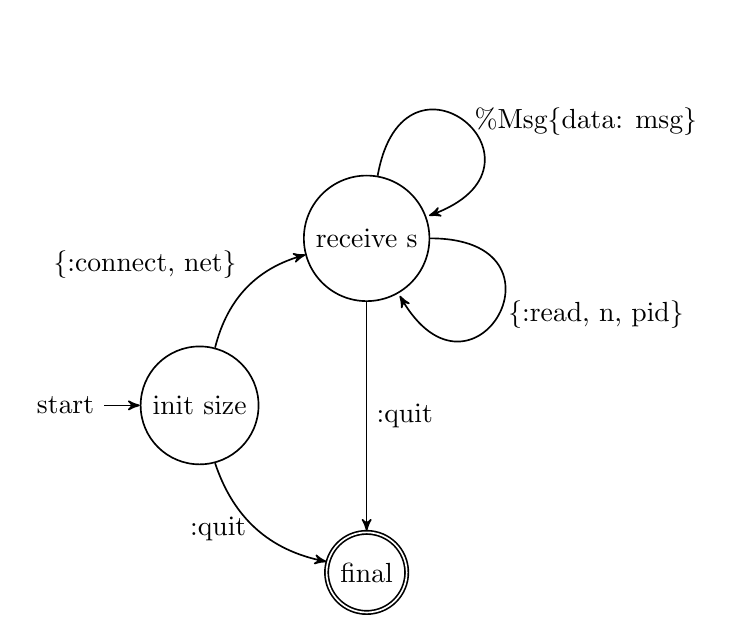
\begin{tikzpicture}[scale=1,>=stealth', node distance=3cm, semithick, auto]
    \node[initial, state]            (init)                              {init size};
    \node[state]                     (receive)   [above right of=init]   {receive s};
    \node[accepting, state]          (final)   [below right of=init]     {final};

    
    \path[->]   (init)   edge  [bend left]     node                  {\{:connect, net\}}        (receive)
                         edge  [below, bend right] node[anchor=east] {:quit}                    (final)
              (receive)  edge  [loop above, every loop/.append style={looseness=6,in=20, out=80 }] node[anchor=west]   {\%Msg\{data: msg\}}   (receive)
                         edge  [loop above, every loop/.append style={looseness=6,in=300, out=0 }] node[anchor=west]   {\{:read, n, pid\}}     (receive)
                         edge  []              node                  {:quit}                    (final);
\end{tikzpicture}}
\subcaption{receiving process}
\end{subfigure}

\caption{The flow control layer.}
\label{fig:flow}
\end{adjustwidth}
\end{figure}


In Fig~\ref{fig:flow} we sea the state diagrams of the sender and
receiver. The sender keeps track of $s$,
the free space in the receiver buffer, a value that is decremented
with each send operation. If this value goes down to $0$
it will enter the {\em ready} state were it must first see a synch
message before it can accept more send operations. 

As with the ordering layer we will implement the sender and receiver
in one Elixir process. We could however have implemented them in
separate processes but we would the of course need two processes on
either side if we want to provide a duplex channel. 

Do as before and implement a test function that creates a sender and a
receiver and connects them over a flow controlled connection.

\section{extensions }

If you think you have everything working you can continue with some
extensions.

\subsection{testing}

Hopefully you have managed so far but let's see if things actually
work. If we tweak our hub a bit we can make it drop a packet every now
and then. As we receive a incoming frame we toss a coin and if we're
unlucky we simply throw the frame away. If things works the ordering
layer should resend the message and also order them in the right
order.

While you at it you can give the hub a {\em loss} rate that
determines how often it should loose a frame. The following code will
get you going:

\begin{minted}{elixir}
  %Frame{} = frm ->
    if :rand.uniform(100) <= loss do
       IO.puts("nub: throwing away #{frm}")
       :ok
    else
       Enum.each(connected, fn({_,pid}) -> send(pid, frm) end)
    end
    hub(loss, connected)
\end{minted}

\subsection{a switch}

Our hub is of course nothing but a hub, it will distribute every frame
in all directions. What would a switch look like?

\subsection{zombies}

By now you probably have a hundred link processes running on you
machine. Every time you test the system you create several processes
that are then not properly terminated. You could of course continue
for a while but if this was a real system we would eventually run out
of resources.

All our processes can take a message {\tt :quit} and should then of
course terminate. The problem is of course to find them, or rather
making sure that who ever started them also terminates them. Since we
want to make sure that processes terminate even if their parent
processes crash we could use linking when processes are
started. Linking is however bi-directional so if a underlying network
process dies it might take it's master process with it.

To solve these problems we could, as in the hub, use monitoring to let
processes detect when their masters die. This soon starts to get
complicated and it should be no surprise that Elixir has a whole
framework, OTP, to handle larger systems.

\subsection{marshaling}

Our link layer can today send anything across the network but this is
not a realistic assumption. Assume that we can only send a byte
sequence. If the interface to the link layer was the message {\tt
  \{:send, string\}}, the layers above would have to encode their
sequence numbers, addresses, packet types etc in a string. This is one
challenge, to encode all data structures as strings before sending
them.

The link layer can now turn into something more interesting and apply
error detection etc to be able to send messages over connections
where bit can be flipped. If you want to learn how a CRC code or a
forward error correction code can be used this is the task to take on.



\newpage
\appendix
\section{linkl.ex} \label{app:link}
\lstinputlisting{src/link.ex}
\pagebreak
\section{hub.ex} \label{app:hub}
\lstinputlisting{src/hub.ex}
\pagebreak

\section{network.ex} \label{app:net}
\lstinputlisting{src/network.ex}
\pagebreak
\section{order.ex} \label{app:order}
\lstinputlisting{src/order.ex}
\pagebreak
\section{frame.ex} \label{app:frame}
\lstinputlisting{src/frame.ex}
\section{netw.ex} \label{app:netw}
\lstinputlisting{src/netw.ex}
\section{ack.ex} \label{app:ack}
\lstinputlisting{src/ack.ex}
\section{ord.ex} \label{app:ord}
\lstinputlisting{src/ord.ex}
\section{syn.ex} \label{app:syn}
\lstinputlisting{src/syn.ex}
\section{msg.ex} \label{app:msg}
\lstinputlisting{src/msg.ex}

\end{document}
